\documentclass[16 pt]{amsart}
\usepackage{amscd,amsmath,amsthm,amssymb}
\usepackage{enumerate,varioref}
\usepackage{epsfig}
\usepackage{graphicx}
\usepackage{mathtools}
\usepackage{tikz}
\usetikzlibrary{graphs,arrows,topaths}
\newtheorem{thm}{Theorem}
\newtheorem{cor}[thm]{Corollary}
\newtheorem{lem}[thm]{Lemma}
\newtheorem{prop}[thm]{Proposition}
\theoremstyle{definition}
\newtheorem{defn}[thm]{Definition}
\theoremstyle{remark}
\newtheorem{ex}[thm]{Example}
\newtheorem{rem}[thm]{Remark}
\numberwithin{equation}{subsection}
\newcommand{\R}{\mathbb{R}}
\newcommand{\Z}{\mathbb{Z}}
\newcommand{\C}{\mathbb{C}}
\newcommand{\Q}{\mathbb{Q}}
\newcommand{\lh}{\lim_{h\rightarrow 0}}
\begin{document}

\title{Exam 3 Maths 140 Spring 2015 \\ DePaul University\\Dr. Alexander}
\maketitle
You have 90 minutes to complete this exam.  Calculators are allowed, but no other electronic devices are permitted.  Please write all your answers in complete, legible sentences, and show all your work to receive full credit.  There are seven (7) problems here.  You may choose to do any 6 of them.  
\vspace{1in}


%table
\begin{center}
  \begin{tabular}{ c | c }
    Problem & Score\\
    \hline
    &\\
    1&\\
    &\\
    2&\\
    &\\
    3&\\
    &\\
    4&\\
    &\\
    5&\\
    &\\
    6&\\
    &\\
    7&\\
    &\\
    Bonus&\\
    &\\
    \hline 
    &\\    
    Total& 
 \end{tabular}
\end{center}

\newpage 

Problem 1. Consider the list of sets 
\[
A_n = \{1,n,n^2\}
\]
Where $n>1$ is an integer.\\

(a) Compute
\[
\bigcup_{n=2}^{5} A_n
\]

(b) Compute
\[
\bigcap_{n=2}^{5} A_n
\]

(c) Compute
\[
\bigcup_{n=2}^{\infty} A_n
\]

\vspace{1in}

Solution: (a) The union $A_2\cup A_3 \cup A_4\cup A_5$ is simply 
\[
\{1,2,3,4,5,9,16,25\}
\]

(b) The only element which is in every set is $1$ and therefore the intersection 
\[
A_2\cap A_3 \cap A_4 \cap A_5 = \{1\}
\]

(c) When taking the infinite union we are assured that each positive integer is in at least one set, namely $n\in A_n$ and this makes the union

\[
\bigcup_{n=2}^{\infty} A_n = \{1,2,3,\dots\}
\]

\newpage

Problem 2. For any two sets $A$ and $B$ define the symmetric difference 
\[
A \Delta B = (A- B)\cup(B- A)
\]

Prove for any three sets $C_1,C_2,C_3$ 
\[
\text{If } C_1\Delta C_3 = C_2\Delta C_3 \text{ then } C_1 = C_2
\]

Hint: Proving this directly is possible, but not the easiest way to go about it.


\vspace{1in}

Solution: Let's prove this with the contrapositive.
Suppose that there are sets $C_1,C_2,C_3$ so that
\[
C_1\Delta C_3 \ne C_2 \Delta C_3
\]
Then we have two options.  Let an element $x\in C_1\Delta C_3$ which is not in $C_2\Delta C_3$.  We are assured that such an $x$ exists since these two sets are not equal.  Then $x\in C_1$ or (exclusive or) $x\in C_3$.
If $x\in C_1$ then $x\notin C_3$ and since $x\notin C_2\Delta C_3$ we see $x\notin C_2$.  Thus, in this case, $C_1\ne C_2$.

On the other hand if $x\in C_3$ then $x\notin C_1$.  Again since $x\notin C_2\Delta C_3$, but $x\in C_3$ this means $x\in C_2$.  So $x\notin C_1$ but $x\in C_2$ and again $C_1\ne C_2$.  This exhausts all possible cases and the proof is complete.

\newpage

Problem 3. Define a map between to sets
\[
F : \Q \rightarrow \Z 
\]
by $F(\frac{a}{b}) = a-b$ 

Explain why $F$ fails to be a function.



\vspace{1in}

Solution: This is not well defined.  Every input has more than one output.  For example
\[
\frac{1}{2} = \frac{2}{4}
\]
but
\[
F(\frac{1}{2}) = 1-2 = -1, \text{ but } F(\frac{2}{4})= 2-4 = -2.
\]
Since $-1\ne -2$ the input $1/2$ has two different outputs and $F$ fails to be a function.


\newpage

Problem 4.  Consider the function
\[
F: \Z \rightarrow \Z
\]
defined by $F(n) = n^3$.

(a) Is this function injective (one to one)?\\

(b) Is this function surjective (onto)?\\

(c) Do either of these properties change if we consider the domain and codomain to be real numbers instead of integers?


\vspace{1in}

Solution: This function is injective since for any two integers $n,m$ we know $n^3=m^3 \iff n=m$.  This is not the case for squares, but for cubes it works.\\

(b) The function is not surjective.  There is no integer so that $n^3=2$.  We miss some integers in the codomain.\\

(c) If we change the domain and codomain to real numbers the injectivity remains, but the function becomes surjective since we can take the cube root of any real number, and it is a real number.  For example $2^{1/3}$ makes perfectly good sense as a real number.



\newpage

Problem 5. Suppose we have 5 fair coins.  If we flip all five coins 

(a) what is the probability of getting exactly two (2) heads?\\

(b) what is the probability of getting two or three (2 or 3) heads?\\

(c) If we flip $n$ coins, what is the probability of getting at least one heads?


\vspace{1in}

Solution: There are 5 coins and therefore 32 total possibilities.  If we count directly, we see that there are 10 possibilities for two heads
\[
HHTTT, HTHTT, HTTHT, HTTTH, THHTT, THTHT, THTTH, TTHHT, TTHTH, TTTHH
\]

So the probability is 
\[
P(\text{exactly 2 heads}) = \frac{10}{32} = \frac{5}{16} \approx 31 \%
\]

(b) Getting three heads exactly is the same as getting exactly two tails.  We know there are ten ways to do this (simply invert all the coins in the previous list).  Therefore we have 20 total ways to get exactly 2 or exactly 3 heads when flipping 5 coins.
\[
P(2 \text{ or } 3 H) = \frac{20}{32} = \frac{5}{8} \approx 61 \%
\]

(c) If we want at least one ``heads" then we can only fail to do this when every coin is ``tails" and so the probability
\[
P(H\ge 1) = \frac{32-1}{32} = \frac{31}{32} \approx 97\%
\] 

\newpage

Problem 6. How many multiples of 7 are in the sequence
\[
546, 547, 548, \dots, 2345 ?
\]


\vspace{1in}

Solution: The smallest multiple is $546 = 7* 78$.  The largest multiple of 7 is $2345=7*335$
Thus we have a list beginning with 78 and ending with 335.  This means there are
\[
335-78+1 = 258
\]
total multiples of 7 in this list.

\newpage

Problem 7. In how many ways can we rearrange the letters of the word
\[
\text{``overnumerousnesses"}?
\]


\vspace{1in}

Solution: There are 18 total letters.  With the following repeats:
\[
(o,2),(e,4),(r,2),(n,2),(u,2),(s,4)
\]
Therefore the total number of arrangements is
\[
\frac{18!}{2!4!2!2!2!4!} = 694702008000	
\]



\newpage

Bonus:  How many triangles in the following picture?


\begin{center}


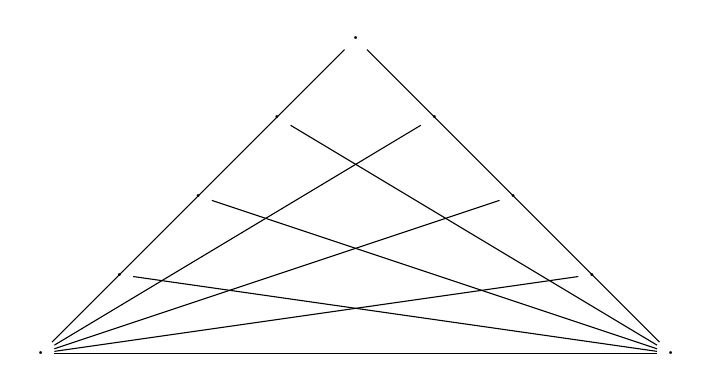
\begin{tikzpicture}
\node (1) at (0,0){.};
\node (2) at (1,1){.};
\node (3) at (2,2){.};
\node (4) at (3,3){.};
\node (5) at (4,4){.};
\node (6) at (5,3){.};
\node (7) at (6,2){.};
\node (8) at (7,1){.};
\node (9) at (8,0){.};
\foreach \from/\to in {1/5,1/6,1/7,1/8,1/9,2/9,3/9,4/9,5/9}
  \draw (\from) -- (\to);
\end{tikzpicture}

\end{center}


\vspace{1in}

Solution: 64. Use the principle of inclusion/exclusion
 

\end{document}